% !TeX spellcheck = cs_CZ
%---------------------------------------------------------------------------------------------------
% file spice.tex
%---------------------------------------------------------------------------------------------------
%================================= Kapitola: Počítačová simulace v elektrotechnice==================
\setchaptertoc
\chapter{Modelování a simulace pomocí SPICE}

  \section{Využití počítače pro návrh obvodů}
    \subsection{Obecný návrhový proces}
      Vývoj nástrojů pro počítačové řešení elektronických obvodů je úzce spojen s vývojem výpočetní
      techniky. Již v průběhu padesátých let minulého století se objevily první programy pro řešení
      velmi specializovaných úloh. Záhy bylo zřejmé, že simulace elektronických obvodů přinese jak
      technické, tak i ekonomické výhody. 
      
      \textbf{Simulací} rozumíme proces, kdy na základě řešení rovnic matematického modelu obvodu
      získáme (přibližnou) informaci o jeho parametrech a charakteristikách. To umožňuje „přeskočit"
      řadu pokusných realizací. Např. v oblasti návrhu integrovaných obvodů je taková realizace
      značně nákladná (stovky tisíc Kč), nemluvě o velmi problematickém měření ve vnitřních uzlech
      obvodu. Některé typy analýz, jako například určení vlivu technologického rozptylu při výrobě,
      je prakticky nemožné uskutečnit. 

      \luagraphic[0.8]{aes_fig008.png}{Obecný postup při návrhu obvodu. 
      (\cite[s.~1]{KolkaBiolek2011})}{aes:fig008}
      
      Velmi zjednodušeně je možné obvyklý proces návrhu obvodu či jakékoli jiné soustavy znázornit
      podle obr. \ref{aes:fig008}. Nazývá se návrh (syntéza) metodou opakované analýzy. Blok č. 1
      představuje oblast s dominantním podílem člověka-návrháře. I přes dflčí pokroky v oblasti
      automatizované syntézy je nepravděpodobné, že bude tuto fázi možné někdy realizovat pouze
      počítačem. To platí zejména pro analogové obvody.

      Celý proces začíná „ručním“ návrhem, kdy na základě požadované funkce a za použití
      jednoduchých vztahů, při zanedbání parazitních jevů, určíme zapojení a přibližné hodnoty
      parametrů obvodových prvků. 
      
      V následujícím kroku je obvod počítačově analyzován za použití mnohem přesnějších modelů,
      které umožní postihnout i všechny významné parazitní jevy. V případě odhalení nesouladu se
      musí provést modifikace navrženého obvodu. Samozřejmě že nedílnou součástí celého procesu musí
      být ověření vlastností navržené soustavy pomocí realizace funkčního vzorku. Snahou je
      minimalizovat počet iterací této vnější smyčky, což vždy přináší úsporu nákladů na vývoj.
      Snaha navrhnout obvod tak, že zvolíme náhodné hodnoty prvků a budeme se pouze pomocí programu
      snažit najít optimum prostřednictvím jejich rozmítání nebo krokování, obvykle k cíli nevede. 
      
      Dominantní oblastí aplikace počítačových metod je numerická analýza (blok č. 2), kdy vstupem
      programu je konkrétní obvod se známými hodnotami prvků a výsledkem jeho charakteristiky. V
      dnešní době, při řešení praktických problémů za použití přesných (a složitých) modelů, není
      možné analýzu provádět ručně nebo graficky. Z hlediska vlastního návrhu plní počítačové
      programy spíše podpůrnou funkci. Výjimku představují programy pro automatizovaná řešení
      některých dílčích úloh, jako je např. návrh analogových kmitočtových filtrů nebo napájecích
      zdrojů.

    \subsection{Programy třídy SPICE}
      V roce 1971 vytvořil student „University of California“, Berkeley, USA \emph{Larry Nagel}
      program \texttt{SPICE1} (\texttt{SPICE} = \emph{Simulation Program with Integrated Circuit
      Emphasis}) v jazyku Fortran. Program umožňoval analýzu dějů v obvodech, obsahujících zejména
      bipolární a unipolární tranzistory. O věrohodnost výsledků bylo usilováno propracovaností
      modelů i matematických algoritmů řešení rovnic. Uživatel měl navíc  možnost
      roz\-ši\-řo\-vá\-ní sortimentu analyzovaných součástek technikou makromodelů zakládáním tzv.
      \emph{pod\-ob\-vo\-dů} (\texttt{subcircuits}) \texttt{SPICE} \cite[s.~2]{KolkaBiolek2011}. 
      
      Protože program byl v podstatě volně šiřitelný, stal se brzo standardním simulačním nástrojem
      pro elektrotechnické úlohy. Usilovně se pracovalo na jeho zdokonalování. V roce 1975 byla
      představena verze \texttt{SPICE2} s podstatně vylepšenými modely i numerickými algoritmy. Tato
      verze byla v průběhu téměř 20 let postupně zdokonalována na Berkeleyské univerzitě až do dnes
      všeobecně známého standardu \texttt{SPICE2G.6}, který byl v r. 1983 zpřístupněn k volnému
      používání. Zdrojové texty \texttt{SPICE1} a \texttt{SPICE2} byly napsány ve Fortranu. Vzhledem
      k zvýšenému využívání unixových pracovních stanic padlo v Berkeley rozhodnutí přepsat SPICE2
      do jazyka C. Tak začala vznikat verze \texttt{SPICE3}. Dnes je rozšířena verze
      \texttt{SPICE3F.5}. Oproti SPICE2G.6 se vyznačuje řadou vylepšení, ovšem z různých důvodů
      došlo k ztrátě zpětné kompatibility se SPICE2G.6. \cite[s.~2]{KolkaBiolek2011}

      S růstem výkonnosti počítačů PC byly programy, dosud běžící na výkonných pracovních stanicích,
      přepisovány na programy spustitelné na „PCčkách“. Tak vznikl standard \texttt{PSpice} (\emph{P
      = počítače PC}). Dnes existuje více simulačních programů, které využívají v podstatě tři ne
      zcela kompatibilní standardy: \texttt{SPICE2}, \texttt{SPICE3}, \texttt{PSPICE}. 
      
      Z hlediska uživatele se mírná odlišnost v syntaxi vstupních souborů projeví zejména při práci
      s modely. Výrobci elektronických prvků obvykle publikují modely ve tvaru \texttt{SPICE2}, aby
      pracovaly ve většině simulátorů. Tím se ovšem nevyužívají možnosti novějších programů. Pokud
      je model napsán ve vyšší verzi, nastávají problémy s nekompatibilitou a text modelu je nutné
      modifikovat.
      
      Z tohoto důvodu se simulátory rozdělují na tzv. „\emph{Spice-like}“ a „\emph{Spice-compatible}
      “simulátory. Označení „\emph{Spice-like}“ znamená, že simulátor je schopen generovat podobné
      výsledky analýzy jako \texttt{SPICE}, avšak nemusí být schopen číst standardní vstupní soubory
      SPICE. Typickými příklady jsou staré verze programů \texttt{Micro-Cap} nebo \texttt{TINA},
      program apod. Termínem „\emph{Spice-compatible}“ se označují simulační programy, které dokáží
      číst standardní vstupní soubory \texttt{SPICE}, provádět klasické \texttt{SPICE} analýzy, a
      generovat výsledky v standardním \texttt{SPICE2G.6} tvaru. Ze současných programů jsou to
      například \texttt{PSpice}, \texttt{HSpice} (standard SPICE3), \texttt{WINSpice} (standard
      \texttt{SPICE3}), \texttt{MicroCap} od verze IV, \texttt{Multisim}, \texttt{LTspice} (standard
      \texttt{SPICE3}) a další.

      Kromě toho existují programy pro simulaci obvodů, které nemají s výše uvedenými skupinami
      programů mnoho společného. Jedná se zejména o jednoúčelové programy, specializované na analýzy
      obvodů, které nelze realizovat programy typu \texttt{SPICE}. Programy typu
      „\texttt{SPICE-compatible}“ jsou široce využívány mimo jiné proto, že umožňují neomezené
      rozšiřování sortimentu modelovaných součástek o nové typy, jejichž modely se průběžně objevují
      na webu a následně i v inovovaných knihovnách nových verzí programů. Na akademických
      pracovištích i v průmyslu je oblíbeným produktem OrcadPSpice. \cite[s.~10]{Biolek2}

      Programy třídy \texttt{SPICE} umožňují tři základní typy analýz. Každá analýza odpovídá
      jistému laboratornímu experimentu, kdy za pomocí signálních generátorů a měřicích přístrojů
      zkoumáme daný obvod. 
      \begin{enumerate}[leftmargin=1cm,rightmargin=.1cm, label=\emph{\alph*}),noitemsep]
        \item \textbf{Analýza v časové oblasti, též přechodová - Transient}: Jedná se o analýzu, kdy
              výsledkem jsou časové průběhy napětí, proudů a z nich odvozených veličin v obvodu.
              Odpovídá laboratornímu experimentu, kdy chování obvodu sledujeme pomocí osciloskopu.
              Kromě napájecích zdrojů mohou být ve schématu i příslušné signální generátory (tj.
              nezávislé zdroje napětí a proudu). 
        \item \textbf{Stejnosměrná analýza - DC}: Předpokládá se, že napětí a proudy se v čase
              nemění, resp. mění tak pomalu, že je můžeme považovat za „stejnosměrné“. Výsledkem
              analýzy je závislost (stejnosměrných) napětí a proudů na nějakém parametru - vstupním
              napětí/proudu, velikosti odporu rezistoru, teplotě, atd. 
        \item \textbf{Střídavá analýza - AC}: Na vstup obvodu je připojen harmonický (sinusový)
              generátor. Předpokládá se, že všechna napětí a proudy jsou harmonické, tj. v obvodu
              dochází pouze k zanedbatelnému zkreslení. Výsledkem jsou amplitudy a fázové posuny
              všech napětí a proudů (komplexní fázory) v závislosti na frekvenci signálu. Tato
              analýza umožňuje zjistit komplexní napěťové přenosy, impedance a admitance. Střídavá
              analýza je použitelná jen pro obvody, které pracují v lineárním režimu, tj.
              zesilovače, kmitočtové filtry, různé přenosové články. Střídavou analýzu nelze použít
              pro obvody, jejichž činnost je založena na využití nelinearity (směšovače, násobiče,
              usměrňovače, atd.).
      \end{enumerate}

      Ostatní analýzy využívají výsledků některé ze základních analýz. Patří k nim
      \textbf{parametrická analýza}, kdy je krokován vybraný parametr (napětí, odpor, teplota,
      atd.). Výsledkem je svazek křivek. \textbf{Citlivostní analýza} poskytuje informace o tom, jak
      změna prvku ovlivní chování obvodu. Např. u oscilátoru můžeme údajem o citlivosti v
      \si{\Hz\per\percent} stanovit, o kolik \si{\Hz} se změní kmitočet při změně parametru
      sledovaného prvku o \SI{1}{\percent}. Analýza \textbf{Monte Carlo} simuluje hromadnou výrobu
      náhodným generováním hodnot parametrů prvků. Pak je možné statisticky vyhodnotit míru
      „výrobního“rozptylu sledovaného parametru. Analýza \textbf{Worst-Case} zjišťuje nejhorší
      možnou kombinaci parametrů prvků v rámci jejich tolerančních intervalů. Obvykle se jedná o
      nadstavbu citlivostní analýzy.

      \subsection{Základní principy obvodové simulace}
        Smyslem počítačové simulace je poskytnutí adekvátní informace o modelované fyzikální
        soustavě pro ověření funkce, resp. další postup návrhu. Forma, jakou je stav obvodu popsán,
        závisí na řešeném problému. Hypoteticky by bylo možné na základě kvantové teorie sestavit
        soustavu rovnic pro pohyb elementárních částic. Z jejího řešení je pak možné odvodit všechny
        další charakteristiky. Je zřejmé, že např. pouhé vykreslení voltampérové charakteristiky
        diody by znamenalo nepřekonatelný výpočetní problém. V dnešní době, i při použití
        nejvýkonnějších počítačů, je možné takto simulovat pouze mikroskopické objekty. Matematický
        model je také možné sestavit s uvažováním např. hustoty nosičů v elementu objemu polovodiče.
        I když bude řešení méně náročné, je proveditelné pro soustavy s maximálně desítkami prvků.
        Nezajímá-li nás dění uvnitř prvku, můžeme pro modelování použít analytické vztahy pro
        svorková napětí a proudy. Pak je možné vyřešit obvody až s desítkou tisíc tranzistorů.

        \luagraphic[1]{aes_fig009.png}{Různé úrovně abstrakce při modelování číslicového obvodu. 
        (\cite[s.~3]{KolkaBiolek2011})}{aes:fig009}

        Hloubka a rozsah informace, získané o objektu, je nepřímo úměrná \emph{úrovni abstrakce}. Na
        obr. \ref{aes:fig009} je znázorněn význam tohoto pojmu. Čím je vyšší úroveň abstrakce, tím
        méně máme informací o jednotlivostech. Na druhou stranu je však možné postihnout větší
        soustavy. Např. na procesor pro stolní počítače se nikdy nedíváme jako na 25 milionů
        tranzistorů, ale jako na systém, který se skládá z bloků (ALU, řadič,...), které dále dělíme
        na registry, hradla, atd. 
        
        Předmětem našeho zájmu bude tzv. \textbf{obvodová simulace}, kdy se obvod modeluje na úrovni
        svorkových napětí a proudů jednotlivých prvků.
      
        \subsubsection{Soustava se soustředěnými parametry}
          Obvod budeme nazývat \emph{soustavou se soustředěnými parametry}, jestliže je možné jej
          rozložit na konečný počet elementárních bloků tak, aby vzájemné energetické interakce
          probíhaly výhradně v konečném počtu idealizovaných bodových svorek - uzlů. Blok může
          představovat jednotlivou součástku nebo větší podsoustavu. Takové dělení je možné
          hierarchicky opakovat.

          \luagraphic[1]{aes_fig010.png}{Rozklad obvodu se soustředěnými parametry. 
          (\cite[s.~3]{KolkaBiolek2011})}{aes:fig010}

          Na obr. \ref{aes:fig010} je znázorněn RC obvod. Ačkoli se spoje mezi prvky kreslí jako
          čáry a nazývají se vodiči, tak soustava takových spojených „vodičů“ představuje uzel -
          bodový objekt, který nemá žádné parazitní vlastnosti. 
          

          Soustavu se soustředěnými parametry můžeme tedy plně popsat souborem prvků a definicí
          vzájemného propojení jejich uzlů, tj. definicí jejich interakcí. Takový popis se nazývá
          slangově netlist (termín převzatý ze simulačních programů). Pro obvod na obrázku by
          netlist standardu \texttt{SPICE} měl tvar:
          \begin{lstlisting}[gobble=8, xrightmargin=13em]
            R1 1 2 1k
            R2 2 0 1k
            C1 2 0 1n
          \end{lstlisting}

          Požadavek na to, aby energie procházela jen přes uzly, není možné fyzikálně splnit. Např.
          pro obvod na obr.\ref{aes:fig010} bude spojení mezi pasivními prvky provedeno pomocí
          plošných spojů. Při připojení střídavého buzení bude k proudům daného uzlu přispívat i
          posuvný proud jeho vlastní (parazitní) kapacity, takže součet proudů přicházejících ze
          svorek jednotlivých prvků nebude zdánlivě roven nule. Stejnou úvahu je možné učinit i o
          napětí indukovaném ve vodiči. Převažuje-li jedna složka pole (např. jen posuvný proud),
          tak je možné do původního obvodu doplnit další prvek (parazitní kapacitu), který bude
          modelovat vlastnosti fyzikálně realizovaného uzlu. Celá soustava tak opět bude mít
          charakter obvodu se soustředěnými parametry a bude plně popsána souborem prvků a definicí
          jejich propojení. Je tedy zřejmé, že pojem \emph{obvodu se soustředěnými parametry} je
          vždy aproximací reality, která nutně přináší chybu. Není-li možné s přijatelnou chybou
          takto obvod řešit, pak musíme použít metody pro \emph{systémy s rozloženými parametry}.

          \luagraphic[1]{aes_fig011.png}{Zahrnutí parazitního prvku (kapacity plošného spoje) do
          modelu obvodu. (\cite[s.~3]{KolkaBiolek2011})}{aes:fig011}

          Na obr. \ref{aes:fig011} je znázorněn proces zahrnutí parazitní kapacity spoje do modelu
          obvodu. V okamžiku návrhu můžeme parazitní vlastnosti spojů pouze odhadnout. Vyžaduje-li
          to povaha úlohy, je možné pomocí speciálního software vypočítat parazitní vlastnosti již
          navrženého např. plošného spoje za účelem provedení ověřovací simulace a eventuální
          korekce návrhu.

        \subsubsection{Modely elektronických prvků}
          \textbf{Modelem} fyzikálního objektu nazýváme reprezentaci tohoto objektu symbolickým
          popisem (rovnicemi) nebo jiným objektem („náhradním schématem“), který z hlediska zkoumaných
          vlastností nahrazuje modelovaný objekt.

          Vzhledem k výhradnímu používání počítačů je modelem elektronického prvku vždy soustava
          rovnic, které říkáme matematický model. Na úrovni obvodové simulace tyto modely popisují
          vztahy mezi svorkovými veličinami (napětí a proudy). V rovnicích vystupují různé
          koeficienty, kterým říkáme parametry modelu.

          Např. matematickým modelem rezistoru (ideálního prvku) je známý vztah
          \begin{equation*}
            u = Ri
          \end{equation*}
          Parametrem tohoto modelu je odpor \(R\).

          \textbf{Identifikací modelu} rozumíme postup pro získání jeho matematického popisu. Velmi
          často se identifikací nazývá pouze proces získání parametrů, když je tvar rovnic předem
          znám.

          \begin{table*}
            \centering
            \begin{tabular}{|p{4cm}|p{4cm}|p{3cm}|}
              \hline
              \rowcolor{CornflowerBlue}{typ}                                & { } & {Model}   \\
              \hline
              rezistor (idealizovaný prvek)             
                & 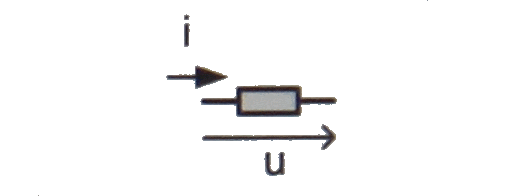
\includegraphics[width=1\linewidth]{aes_fig012a.png}      & \(u = Ri\)      \\
              \hline
              rezistor (model pro vyšší frekvence)      
                & 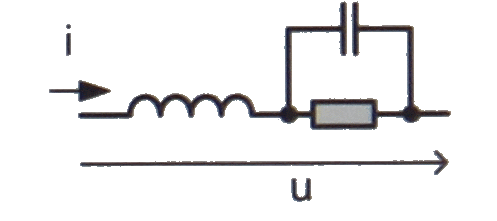
\includegraphics[width=1\linewidth]{aes_fig012b.png}      
                & náhradní schéma tvořené elementárními prvky \\ 
              \hline    
              nelineární prvek - varistor               
                & 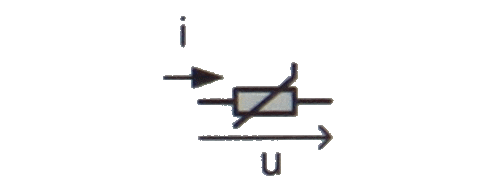
\includegraphics[width=1\linewidth]{aes_fig012c.png}      & \(i = Au^B\)    \\
              \hline
              polovodičová dioda (elementární model)    
                & 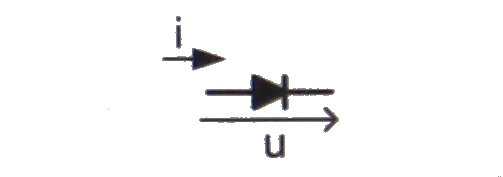
\includegraphics[width=1\linewidth]{aes_fig012d.png} 
                &  \(i = I_s\left(e^\frac{u}{nV_T}-1\right)\)  \\
              \hline 
            \end{tabular}
            \caption{Příklady modelů}\label{aes:tab001}
          \end{table*}

          Matematický model celého obvodu vznikne sloučením modelů dílčích prvků s Kirchhoffovými
          rovnicemi, které popisují interakce mezi prvky. Výsledkem je soustava tzv.
          \emph{algebraicko-diferenciálních rovnic}. Běžný uživatel simulačního programu, na rozdíl od
          jeho tvůrce, se s těmito rovnicemi přímo nesetká.

      \subsection{Simulace a realita}
        Přes všechen pokrok v oblasti počítačové podpory návrhu však dosud neexistuje program, do
        něhož by uživatel zadal obvod (schéma) a po stisknutí tlačítka obdržel důvěryhodné výsledky,
        aniž by o obvodu něco věděl. Výsledky mohou být chybné a je jen na uživateli, aby je kriticky
        posoudil. 
        
        Příčiny nesouladu mezi realitou a simulací můžeme rozdělit do čtyř kategorii:
        \begin{enumerate}[leftmargin=2cm,rightmargin=0.8cm, label=\emph{\alph*}),noitemsep]
          \item chyby vzniklé při vlastním řešení rovnic obvodového modelu v simulátoru, 
          \item nepřesné modely,
          \item výrobní rozptyl, 
          \item zanedbané parazitní prvky.
        \end{enumerate}

        \begin{itemize}[noitemsep]
          \item \textbf{Chyby simulátoru}: Při numerickém řešení soustavy rovnic, popisující obvod,
                vznikají chyby zaokrouhlováním, diskretizací i iteračním způsobem řešení.
                Pomineme-li problémy prvků popsaných ve frekvenční oblasti a tzv. špatně podmíněné
                úlohy, tak je možné říci, že přesnost výpočtu má uživatel pod kontrolou
                prostřednictvím parametrů RELTOL, ABSTOL a VNTOL (\todo[inline]{blíže v kap. 1.4.2.1}).
                Obvykle je nastavena relativní chyba \SI{0.1}{\percent}. Požadování vyšší přesnosti
                zpomalí simulaci nebo může v krajním případě vést k jejímu selhání. Je také
                diskutabilní, zdali požadovat výrazně vyšší přesnost simulace, než mohou mít měřicí
                přístroje v laboratoři. 
          \item \textbf{Nepřesné modely}: Každý model je jen aproximací reality. Používané modely
                jsou kompromisem mezi požadavkem na přesnost, výpočetní efektivitu a možnost snadné
                identifikace parametrů na základě měření.
          \item \textbf{Výrobní rozptyl}: Výrobní rozptyl je značný zejména u polovodičů. Např.
                proudový zesilovací činitel bipolárního tranzistoru může mít toleranci až
                \SI{\pm50}{\percent}.
          \item \textbf{ Odhad parazitních prvků}: Dalším problémem jsou parazitní vlastnosti
                propojovacích vodičů mezi prvky. To, co je nakresleno v editoru schématu jako vodič,
                vlastně představuje ideální spoj bez parazitní indukčnosti, odporu i kapacity.
                Zvláště při analýze obvodů v megahertzové oblasti vyžaduje odhad parazitních prvků i
                jistou zkušenost s praktickou realizací. Při neuvažování parazitních prvků vlastně
                analyzujeme neúplný model obvodu.                          
        \end{itemize}
        \begin{mdframed}[style=mdnote]
          \begin{note}
            Vliv výrobního rozptylu si ukažme na příkladu (nevhodného) nastavení pracovního body
            zesilovače v zapojení \texttt{SE}. Zapojení je velmi citlivé na parametry tranzistoru.
            Předpokládejme, že máme konkrétní kus tranzistoru \texttt{Philips/NXP BC546A}, který
            změříme a na základě změřených hodnot vytvoříme model. V tom případě bude chyba mezi
            simulací a měřením např. kolektorového proudu řádu procent.
            
            {\centering
            \captionsetup{type=figure}
              \subcaptionbox{\label{aes:fig013a}}{\luafigure[.45]{aes_fig013a.png}} 
              \hspace{1em} 
              \subcaptionbox{\label{aes:fig013b}}{\luafigure[.45]{aes_fig013b.png}}  
            \captionof{figure}{a) Nastavení pracovního bodu; b) model a skutečné prvky 
                       (\cite[s.~6]{KolkaBiolek2011})
            \label{aes:fig013}}
           \par}

          Uvažme nyní, že použijeme jiný kus téhož typu a stále stejný model. Podle údajů
          katalogového listu leží proudový zesilovací činitel \(h_{21E}(\beta)\) v rozmezí \num{110}
          až \num{220}. U druhého tranzistoru bude parametr h21e jiný, dopředu neznámý. I kdybychom
          vytvořili dokonalý model pro první tranzistor, tak při použití druhého tranzistoru
          dostaneme odchylku v řádu desítek procent.

          V praxi se navíc vytvářejí modely spíše pro typické hodnoty, které ani nemusí popisovat
          konkrétní existující kus. Na obr. \ref{aes:fig013b}  je to ilustrováno graficky (pro
          případ, kdyby měl model jen dva parametry). Je tedy zřejmé, že otázka: \uv{Jakou hodnotu
          bude mít kolektorový proud?} je nesprávně položena. Správně položená otázka zní: \uv{V
          jakém rozsahu se může nacházet kolektorový proud, když uvážíme výrobní rozptyl všech
          prvků?} Pak teprve můžeme porovnávat simulaci a realitu.

          Musíme se tedy smířit s tím, že model vždy vyjadřuje jen parametry jednoho (hypotetického)
          prvku. Dobrý model musí navíc věrně postihovat např. závislost parametrů na teplotě,
          frekvenci, nebo kolektorovém proudu.
        \end{note} 
      \end{mdframed} 

  \section{Modelování základních obvodů}
    \subsection{Typické uspořádání simulačních programů}
      Pojem \texttt{SPICE} označuje vlastní výpočetní jádro, které řeší obvodové rovnice. Moderní
      simulátory jsou obvykle součástí větších systémů pro kompletní návrh klasických nebo
      integrovaných obvodů.

      Bohužel standard \texttt{SPICE} není zaštítěn žádnou respektovanou organizací. Proto existují
      mezi jednotlivými programy drobné rozdíly v syntaxi vstupních souborů. Knihovny a vytvořené
      obvody obvykle nejsou automaticky plně přenositelné. Většinou programy zachovávají zpětnou
      kompatibilitu se syntaxí použitou ve \texttt{SPICE2} a \texttt{SPICE3}. Pokud např. výrobci
      prvků poskytují (na Internetu) modely, tak v naprosté většině právě v kompatibilní formě. To
      má za následek, že se nevyužijí možnosti, které byly přidány do různých komerčních variant
      \texttt{SPICE}.

      Na obr. \ref{aes:fig014} je ustálené uspořádání simulačního programu. Systém obvykle obsahuje
      tři moduly: \emph{editor schématu}, \emph{simulátor} a \emph{postprocesor} - modul pro
      vykreslování výsledků analýzy a jejich další zpracování. Editory schématu a postprocesory se
      od jednotlivých výrobců velmi výrazně odlišují. Z pohledu uživatele má největší význam to, že
      rozhraní editor + simulátor je víceméně standardizované. Právě tomu se říká „standard SPICE“.
      Informace o obvodu a požadovaných analýzách jsou simulátoru předávány pomocí textových
      souborů. Přenositelnost jak obvodů, tak knihoven modelů je zajištěna právě na úrovni těchto
      souborů. To je důvod, proč se všechny obvody a modely publikují jako textové soubory. Formáty
      souborů pro uložení schématu jsou většinou neveřejné, často podléhající licenci.

      \luagraphic[1]{aes_fig014.png}{Typické uspořádání simulačního programu. 
      (\cite[s.~8]{KolkaBiolek2011})}{aes:fig014}      

      Na obr. \ref{aes:fig015} je příklad organizace souborů pro stejnosměrnou analýzu jednoduchého
      obvodu s diodou, kdy napětí stejnosměrného zdroje je rozmítáno od \SI{-3}{\V} do \SI{+3}{\V}.
      Vstupní soubor je vygenerován automaticky editorem schématu nebo může být editován ručně.
      První část tvoří popis samotného obvodu. Každému prvku odpovídá jeden řádek. Parametry zdroje
      napětí (\texttt{V\_V1}) a rezistoru (\texttt{R\_R1}) jsou plně popsané v netlistu. Uzly jsou
      ve schématu očíslované jako \num{1} a \num{2}, referenční uzel je vždy \num{0}. Dioda je
      popsána složitým modelem s mnoha parametry, který je uložen v knihovně spolu s dalšími modely.
      Řádek v netlistu obsahuje jen odkaz na model.

      \luagraphic[1]{aes_fig015.png}{Struktura vstupních souborů.
      (\cite[s.~9]{KolkaBiolek2011})}{aes:fig015}      

      Jméno knihovního souboru je uvedeno v příkazu \texttt{.LIB}. V poslední části jsou příkazy pro
      rozmítání stejnosměrné složky \(V_1\) s krokem \SI{50}{\mV}. Příkaz \texttt{.PROBE} určuje, že
      napětí obou uzlů se budou ukládat pro zpracování v postprocesoru (zobrazení grafů). Model z
      knihovny (příkaz \texttt{.model...}) může být umístěný v hlavním souboru. V tom případě
      knihovnu nepotřebujeme a celá úloha je definovaná jen jedním souborem. Tento styl je výhodný,
      pokud někomu potřebujeme poskytnout náš \uv{obvod} v textové formě. Netlistem by se měl
      nazývat jen soupis prvků. Někdy se tak ovšem říká i celému vstupnímu souboru, obsahujícímu
      také příkazy.
      
      \begin{mdframed}[style=mdnote]
        \begin{note}
          Uživatel simulačního programu je prakticky vždy nucen pracovat i s textovými soubory
          knihoven nebo netlistů, například při zahrnování nového modelu do knihovny nebo hledání
          chyb podle hlášení simulátoru.
        \end{note}
      \end{mdframed}

      Vstupní soubor z obr. \ref{aes:fig015} je možné \uv{odsimulovat} programem
      \texttt{PSpice}. Hlavní textový soubor nazveme např. jako \texttt{obvod.cir}
      a knihovnu jako \texttt{diody.lib} (text lze zkopírovat přes schránku Windows). Spustíme
      program \texttt{PSpiceAD} (nikoli editor schématu \texttt{Capture}). Zvolíme
      \texttt{File/Open} a nastavíme typ souboru na \texttt{*.cir}. Volbou \emph{Simulation/Run} se
      spustí analýza. Po skončení se pomocí \texttt{Trace/Add Trace} zobrazí např. průběh \(v(2)\) -
      napětí na diodě. \todo[inline]{Podrobnosti viz kapitola 1.2.4 na str. 20.s}

    \subsection{Základní pravidla jazyka (P)Spice}
      Kromě definice struktury obvodu a modelů prvků obsahuje vstupní soubor i příkazy pro simulátor
      k provádění různých analýz, ukládání výsledků a nastavování parametrů algoritmů pro numerické
      řešení.

      \begin{mdframed}[style=mdnote]
        \begin{note}
          Syntaktická pravidla:
          \begin{itemize}[noitemsep]
            \item První řádek vždy slouží jako hlavička (nadpis),
                  \texttt{PSpice} jej ignoruje\footnote{na obr. \ref{aes:fig015} je to
                  řádek: \texttt{* obvod}}. 
            \item Prázdné řádky, vícenásobné mezery a další „bílé znaky“ se ignorují. 
            \item Malá a velká písmena se nerozlišují. 
            \item Na pořadí řádků nezáleží (s výjimkou prvního a posledního řádku). 
            \item Názvy všech obvodových prvků musí být jedinečné. 
            \item Každý řádek (s výjimkou hlavičky) začíná jedním z těchto symbolů: 
                  \begin{itemize}[noitemsep]
                    \item \textbf{znak 'A' až 'Z'} - definice obvodového prvku (např. R pro
                          rezistor\footnote{Jednotlivé verze SPICE se mohou mírně lišit v přiřazení
                          znaků k prvkům.}).
                    \item \textbf{znak '*'} - obsah řádku je chápán jako komentář. 
                    \item \textbf{znak '+'} - řádek je pokračováním předchozího
                          řádku\footnote{Používá se pro zlepšení čitelnosti.}. 
                    \item \textbf{znak '.'} - příkaz simulátoru (např. \texttt{.DC} provede
                          stejnosměrnou analýzu).
                  \end{itemize}
            \item Vše, co je napravo od znaku středník ';', je chápáno jako komentář.
            \item Soubor končí příkazem \texttt{.END}. 
            \item Uzly se značí alfanumerickým řetězcem bez mezer. Původní standard dovoloval jen
                  označení celými čísly. Jeden z uzlů musí být označen jako O (nula).
            \item Čísla se zapisují v přirozeném tvaru (\num{0.25}) vždy s desetinnou tečkou, v
                  exponenciálním tvaru (1e-3), nebo je možné použít standardní technické přípony
                  (\texttt{f, u, m, k, meg, g, t}). Mezi číslem a příponou se nesmí psát mezera.
                  Ostatní znaky za číslem se ignorují (\texttt{1uF = 1u}). Přípona \texttt{m} i
                  \texttt{M} znamená \texttt{mili} (\num{e-3}) - nerozlišují se malá a velká
                  písmena. 
            \item Od \texttt{PSpice} verze 15 je možné využívat i tzv. Evropský způsob, kdy se
                  přípona píše místo desetinné tečky. Např. \texttt{4k7 = 4.7k}. Místo desetinné
                  tečky je také možné použít \texttt{R} pro rezistory, \texttt{L} pro induktory a
                  \texttt{C} pro kapacitory. Např. \texttt{1R2 = \SI{1.2}{\ohm}}, ale jen u
                  rezistoru.
          \end{itemize}
        \end{note}
      \end{mdframed}

      \subsubsection{Definice prvků}
        Řádek netlistu, který definuje obvodový prvek, začíná pevně daným znakem. Jednotlivé
        varianty \texttt{SPICE} se mohou v přiřazení znaků mírně odlišovat. V programu
        \texttt{PSpice} jsou definovány tyto prvky: 

  \section{Základní analýzy}
    \subsection{Stejnosměrná analýza}
      Stejnosměrná analýza odpovídá laboratornímu experimentu, kdy např. na vstup obvodu připojíme
      regulovatelný stejnosměrný zdroj a měříme závislost výstupního stejnosměrného napětí na
      vstupním. V podstatě se jedná o sledování závislosti stejnosměrného pracovního bodu na nějaké
      veličině (napětí, proud, odpor, teplota, atd.).

      \luagraphic[1]{aes_fig019.png}{Stejnosměrná analýza.
      (\cite[s.~59]{KolkaBiolek2011})}{aes:fig019}         


      Hledání pracovního bodu si vysvětlíme na příkladu \emph{Colpittsova oscilátoru} z obr.
      \ref{aes:fig020a}. První krok spočívá v odstranění setrvačných prvků z obvodu, protože ty
      nemají na stejnosměrný pracovní bod vliv. Induktory jsou nahrazeny zkratem a kapacitory jsou
      jednoduše vypuštěny. Po odstranění setrvačných prvků zmizí z obvodových rovnic čas. Standardní
      stejnosměrná analýza proto nemůže poskytnout informaci o stabilitě či nestabilitě pracovního
      bodu. Při laboratorním měření však nelze z obvodu nikdy odstranit setrvačnost (přinejmenším ne
      parazitní prvky). Aby bylo možné měření provést, musí být u reálného systému pracovní bod
      samozřejmě stabilní. (V literatuře byly popsány metody pro odhad stability bez znalosti
      setrvačných prvků - zatím se však v praxi nepoužívají.)

      \begin{figure}[ht!]
        \centering  
        \subcaptionbox{\label{aes:fig020a}}{\luafigure[0.9]{aes_fig020a.png}}          \newline
        \subcaptionbox{\label{aes:fig020b}}{\luafigure[0.5]{aes_fig020b.png}}               
        \caption{Úprava obvodu pro výpočet pracovního bodu. (\cite[s.~59]{KolkaBiolek2011})}
        \label{aes:fig020}
      \end{figure}

      Pracovní bod je charakterizován stejným napětím na kolektoru a bázi bipolárního tranzistoru,
      protože tyto svorky jsou stejnosměrně propojené přes indukčnost \(L\). Rozpojme nyní tyto
      svorky. Napětí báze je označeno jako \(U_1\), napětí kolektoru pak jako \(U_2\). Na obr.
      \ref{aes:fig021a} je znázorněna závislost \(U_2=f(U_1)\). Jedná se vlastně o zesilovač v
      zapojení \texttt{SE}. Pracovní bod se nachází tam, kde platí \(U_1 = U_2\). Na druhém grafu je
      vynesena závislost \(U_1-U_2\). V pracovním bodu tedy musí platit \(U_1 - U_2 = 0\). Hledáme
      průsečík zobrazené křivky s nulou.

      \begin{figure}[ht!]
        \centering  
        \subcaptionbox{\label{aes:fig021a}}{\luafigure[0.40]{aes_fig021a.png}}    \hspace{1em}
        \subcaptionbox{\label{aes:fig021b}}{\luafigure[0.45]{aes_fig021b.png}}               
        \caption{Princip výpočtu pracovního bodu. (\cite[s.~60]{KolkaBiolek2011})}
        \label{aes:fig021}
      \end{figure}
      
      U všech programů třídy \texttt{SPICE} je výpočet pracovního bodu prakticky shodný. Používá se
      \textbf{Newton-Raphsonova metoda tečen}. Její princip si můžeme představit podle obr.
      \ref{aes:fig021b}. Metoda hledá kořen algebraické rovnice, tj. \emph{průsečík nějaké
      funkce s osou \(x\)}. Výpočet probíhá vždy iteračně. Na počátku je nutné zvolit výchozí bod
      \(U_1^{(0)}\), ve kterém se určí tečna. Její průsečík s osou \(x\) dává nový bod (odhad
      kořene) \(U_1^{(1)}\), pak \(U_1^{(2)}\), atd.. Celý proces se iteračně opakuje. V dalších
      krocích se program blíží k průsečíku - hledanému pracovnímu bodu, který však nikdy přesně
      nedosáhne. Iterace jsou zastaveny, až chyba klesne na přijatelnou hodnotu nebo až je překročen
      maximální povolený počet iterací. V případě existence více pracovních bodů (křivka má více
      průsečíků s osou) nalezne metoda vždy jen jeden pracovní bod v závislosti na zvoleném výchozím
      bodu. Pro některé úlohy mohou iterace divergovat (vzdalují se od průsečíku). V takovém případě
      program oznámí, že pracovní bod nebyl nalezen.

      \begin{mdframed}[style=mdnote]
        \begin{note}
          Vlastnosti metody použité pro výpočet pracovního bodu je možné formulovat do následujících
          bodů:
          \begin{itemize}[noitemsep]
            \item Nalezení pracovního bodu není garantováno. Problémy se mohou vyskytnout u obvodů s
                  vysokým ziskem (operační zesilovače) nebo s ostrými nelinearitami (příliš
                  idealizované behaviorální modely).
            \item Čím lépe odhadneme výchozí bod, tím rychlejší a spolehlivější bude konvergence. 
            \item V případě existence více pracovních bodů najde metoda vždy jen jeden v závislosti
                  na výchozím bodu. 
            \item Řešení neposkytne informaci o stabilitě nalezeného pracovního bodu.
          \end{itemize}
        \end{note}
      \end{mdframed}    

    \subsection{Analýza v časové oblasti}
      Analýza odpovídá laboratornímu experimentu, kdy obvod, na jehož vstup je připojený signální
      generátor, měříme osciloskopem. Výsledkem analýzy jsou časové průběhy napětí a proudů v
      obvodu.

      \luagraphic[1]{aes_fig016.png}{Výsledky časové analýzy.
      (\cite[s.~68]{KolkaBiolek2011})}{aes:fig016}  

      Řešení v simulátoru probíhá vždy tak, že obdržíme všechny průběhy \(u(t)\) a \(i(t)\)
      vzorkované v diskrétních časech \(t_i\), přičemž dělení časové osy není ekvidistantní.

      Časový krok si program volí automaticky podle aktuální strmosti průběhu veličin v obvodu a
      požadované přesnosti výpočtu. Při pomalých změnách se prodlužuje a při prudkých změnách
      zkracuje. Délka kroku se automaticky nastavuje tak, aby program stále počítal s přibližně
      stejnou chybou. Při pevném kroku by jeho velikost musela být nastavena podle „rychlých“ úseků.
      V úsecích s „pomalou“ změnou by malý krok zbytečně zvyšoval výpočetní náročnost, nehledě na
      akumulaci numerických chyb.

      Na obr. \ref{aes:fig017} je znázorněn algoritmus pro řízení kroku v závislosti na charakteru
      signálů. V případě pomalých změn napětí a proudů se volí velký krok. Pokud se mezi dvěma kroky
      objeví např. strmá nástupní hrana vstupního signálu, tak v čase \(t_3\) vznikne
      neakceptovatelně velká chyba (to se zjistí až po výpočtu tohoto kroku). Řešení v čase \(t_3\)
      musí být zamítnuto. Program se vrátí do \(t_2\) a pokračuje s menším krokem, např. polovičním.
      Proces zkracování kroku pokračuje tak dlouho, dokud se nedosáhne akceptovatelné chyby. Naopak
      pokud řešení probíhá s chybou menší než je povolená hodnota, tak se krok prodlužuje.

      
      \luagraphic[1]{aes_fig017.png}{Princip automatické volby časového kroku.
      (\cite[s.~68]{KolkaBiolek2011})}{aes:fig017}  

      Dynamická změna kroku má ovšem své meze. Shora je krok omezen délkou intervalu, na kterém
      probíhá řešení tak, aby výsledkem byl „rozumný“ počet bodů, ze kterého je možné sestavit graf
      (např. \num{50} až \num{100} hodnot). Zdola je krok omezen přesností zobrazení čísel v
      počítači. Předpokládejme, že je čas v simulátoru reprezentován proměnnou typu double s
      přesností \num{15} míst. Pokud by např. došlo ke zkrácení kroku z důvodu velmi strmé hrany na
      \(\Delta t = \num{e-20}\) v čase \(t = \SI{1}{\second}\), tak nový časový okamžik bude opět
      \(\num{1} + \num{e-20} \approx 1\), protože je čas reprezentován omezeným počtem míst. Výpočet
      by se proto zastavil. Pro krok je možné formulovat podmínku

      \begin{equation}\label{aes:eq024}
        \frac{T_{max}10^{-m}}{tol} \leq h \leq \frac{T_{max}}{N}, 
      \end{equation}

      kde \(T_{max}\) je délka simulačního simulačního intervalu. \(N\) bývá v rozsahu \num{50} až
      \num{100}, \(m\) je počet platných míst (\num{15} pro \emph{double} a \(tol\) je povolená
      relativní chyba zobrazení času (např. \num{e-3}).

      Není-li možné dodržet předepsanou chybu výpočtu při splnění podmínky (\ref{aes:eq024}), tak je
      řešení ukončeno. Potom je nutné provést změny v samotném obvodu, nastavení analýzy nebo
      globálních podmínek simulátoru. Následující odstavec uvádí některá doporučení, založená na
      praktických zkušenostech uživatelů:

      \begin{mdframed}[style=mdnote]
        \begin{note}
          \begin{itemize}[noitemsep]
            \item Používat spojité a hladké funkce při vytváření modelů. Doplnit nelinearitu o
                  parazitní kapacitu (paralelně ke zdroji proudu) či indukčnost (sériově ke zdroji
                  napětí).
            \item Zmenšit délku simulačního intervalu, snížit požadavek na přesnost. 
            \item Nepoužívat ideální impulzní signály (s nulovou délkou hrany). Např. ideální
                  jednotkový skok není stejně možné v praxi realizovat. Nastavíme-li délku hrany o
                  \num{4} řády kratší než je nejmenší časová konstanta v obvodu (stačí odhad), tak
                  dostaneme číselně stejný výsledek jako pro ideální signál.
          \end{itemize}
        \end{note}
      \end{mdframed}

      \subsection{Stabilita integrační metody}
        Při numerickém řešení v časové oblasti se \emph{soustava algebraicko-diferenciálních rovnic}
        (spojitý čas) matematického modelu obvodu převádí na \emph{soustavu diferenčních rovnic}
        (diskrétní čas). Při tomto převodu nastávají problémy se \textbf{stabilitou}. Je přirozené, že
        při analýze stabilního obvodu potřebujeme, aby simulovaná odezva byla také stabilní a výsledky
        tak odpovídaly realitě. Tento požadavek však není splněn automaticky mimo jiné proto, že
        závisí na typu řešené úlohy. Aby bylo možné srovnávat jednotlivé metody, používá se standardně
        testovací diferenciální rovnice prvního řádu ve tvaru
        \begin{equation}\label{aes:eq025}
          \dot{x} = \lambda x, 
        \end{equation}
        kde \(\lambda\) je komplexní kořen charakteristické rovnice (v případě přenosu by to byl
        pól). Přesné řešení rovnice je ve tvaru \(x(t) = C\exp(\lambda t)\). Rovnovážný stav \(x =
        0\) je stabilní, pokud \(\realset(\lambda)\leq0\). Stabilita numerického řešení se
        vyhodnocuje zobrazením součinu \(\Delta t\lambda\) (\(\Delta\) je \emph{časový krok}) do
        komplexní roviny. Protože časový krok je vždy kladný, \(\Delta t>0\), tak bychom u ideální
        metody čekali, že bude poskytovat stabilní \emph{numerické} řešení pro všechna
        \(\Delta t\lambda\) ležící v levé polorovině, viz obr. \ref{aes:fig018a}. Tuto vlastnost
        splňuje pouze tzv. \textbf{lichoběžníková metoda}, u které se však projevují parazitní
        zákmity při analýze impulzních obvodů. Z toho důvodu se více používají metody, které tuto
        vlastnost nemají.

        \begin{figure}[ht!]
          \centering  
            \subcaptionbox{\label{aes:fig018a}}{\luafigure[0.45]{aes_fig018a.png}}  \hspace{1em}            
            \subcaptionbox{\label{aes:fig018b}}{\luafigure[0.45]{aes_fig018b.png}}  \newline            
            \subcaptionbox{\label{aes:fig018c}}{\luafigure[0.45]{aes_fig018c.png}}  
          \caption{Oblast absolutní stability a) lichoběžníková metoda; b), c) Gearova metoda}
          \label{aes:fig018}
        \end{figure}

        Jedna z nejrozšířenějších metod, která je využita i v \texttt{PSpice}, je tzv.
        \textbf{Gearova metoda}. Na obr. \ref{aes:fig018b} a \ref{aes:fig018c} jsou
        vyznačené oblasti její stability. Řád metody (tj. stupeň polynomu, který lokálně aproximuje
        řešení) se automaticky mění podobným způsobem jako časový krok. Při zkracování kroku se
        používá nižší řád a naopak.

        Pro řád \num{2} vidíme, že metoda poskytuje stabilní řešení i v případě, že kořen (pól) leží
        v pravé polorovině! Naopak pro řád \num{5} poskytuje nestabilní řešení i v případě, že kořen
        (pól) leží v levé části komplexní poloroviny. Tím se stává problematickým použití časové
        simulace pro odhalení nestability, zvláště v případech, kdy kořeny (póly) leží blízko
        imaginární osy.

        \subsection{Střídavá analýza}

        \luagraphic[1]{aes_fig022.png}{Výsledky střídavé analýzy - modulová charakteristika v
        \si{\decibel}. (\cite[s.~79]{KolkaBiolek2011})}{aes:fig022}  

        \luagraphic[1]{aes_fig023.png}{Výpočet střídavé odezvy integračního článku.
        (\cite[s.~79]{KolkaBiolek2011})}{aes:fig023}  

        
  \section{Simulace a analýza v programu LTspice IV}
   
  \section{Příkazy pro řízení simulace}
    
    \begin{figure}[ht!]
      \centering
      \subcaptionbox{\label{SPICE:fig_ltc001_Ra}}{\luafigure[0.45]{../ltspice/ltc001_RC.pdf}}
      \subcaptionbox{\label{SPICE:fig_ltc001_Rb}}{\luafigure[0.45]{../ltspice/CompAttrEditor.png}}  
      \caption{\texttt{ltc001\_RC.asc}: Nastavení počáteční velikosti napětí na které je 
               kondenzátor nabit}
      \label{SPICE:fig_ltc001}
    \end{figure}

  \section{Úvod do simulace spínaných napájecích zdrojů}
    % In the electronics world, different types of circuitries must cohabit: logic devices, analog 
    % circuits, microprocessors, and so on. Unfortunately for the designer, these circuits do not 
    % cope with a single, fixed, power supply rail: A microprocessor or a digital signal processor 
    % (DSP) will need a stable 3.3-V source or less, a front-end acquisition board will require ±15 
    % V and perhaps some logic glue around a standard 5 V. For the final board being supplied from 
    %%% a single power point, for example, the mains outlet or a battery, how is one to adapt and 
    % distribute all these different voltages to the appropriate portions? The solution consists of 
    % inserting a so-called converter to adapt the voltage distribution to the circuit needs.
    
    Ve světě elektroniky (obr. \ref{SPICE:Basso_intro}), musí různé druhy elektronických obvodů 
    vzájemně spolupracovat (logické obvody, analogové obvody, mikroprocesory, atd.). Bohužel tyto 
    obvody nepracují s jediným napájecím napětím: mikroprocesor nebo signálový procesor (DSP), bude 
    potřebovat například zdroj \SI{3.3}{\volt}, analogové obvody mohou vyžadovat symetrické nápení 
    \SI{\pm15}{\volt}. Ovšem externí napájecí zdroj je zpravidla jen jeden (např. síťové napájení 
    \SI{230}{\volt}, baterie). Vzniká tak otázka, jakým způsobem z tohoto zdroje realizovat tolik 
    napájecích úrovní. Řešení spočívá ve vložení tzv. převodníku mezi zdroj a napájený obvod, který 
    přizpůsobí napájecí napětí konkrétním požadavkům obvodu.
    
    \begin{figure}[ht!]
      \centering
      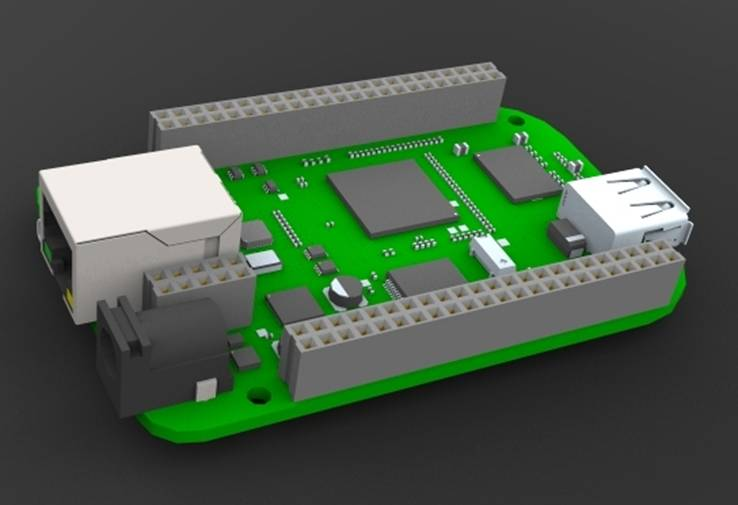
\includegraphics[width=0.6\linewidth]{beaglebone.jpg}
      \caption{Příklad plošného spoje s mnoha druhy integrovaných obvodů, vyžadující odlišné 
               napájecí úrovně}
      \label{SPICE:Basso_intro}
    \end{figure}

%---------------------------------------------------------------------------------------------------